\documentclass[border=4pt]{standalone}
\usepackage{tikz}
\usetikzlibrary{arrows.meta,calc,positioning}

\begin{document}
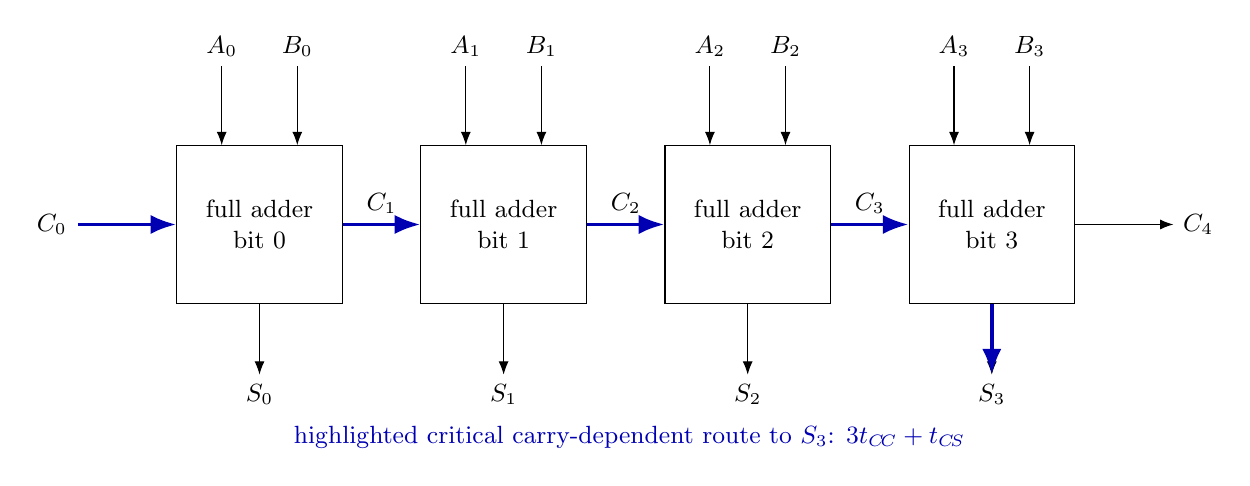
\begin{tikzpicture}[
  >=Latex,
  font=\small,
  fa/.style={draw,minimum width=2.1cm,minimum height=2.0cm,align=center},
  carry/.style={->,blue!70!black,line width=1.4pt}
]
  \node[fa] (FA0) at (1.4,1.8) {full adder\\bit 0};
  \node[fa] (FA1) at (4.5,1.8) {full adder\\bit 1};
  \node[fa] (FA2) at (7.6,1.8) {full adder\\bit 2};
  \node[fa] (FA3) at (10.7,1.8) {full adder\\bit 3};

  \foreach \nodeid/\i in {FA0/0,FA1/1,FA2/2,FA3/3} {
    \draw[->] ($(\nodeid.north)+(-0.48,1.0)$)
      node[above] {$A_{\i}$} -- ($(\nodeid.north)+(-0.48,0)$);
    \draw[->] ($(\nodeid.north)+(0.48,1.0)$)
      node[above] {$B_{\i}$} -- ($(\nodeid.north)+(0.48,0)$);
    \draw[->] (\nodeid.south) -- ++(0,-0.9)
      node[below] {$S_{\i}$};
  }

  \draw[carry] ($(FA0.west)+(-1.25,0)$)
    node[left,black] {$C_0$} -- (FA0.west);
  \draw[carry] (FA0.east) -- (FA1.west)
    node[midway,above,black] {$C_1$};
  \draw[carry] (FA1.east) -- (FA2.west)
    node[midway,above,black] {$C_2$};
  \draw[carry] (FA2.east) -- (FA3.west)
    node[midway,above,black] {$C_3$};
  \draw[->] (FA3.east) -- ++(1.25,0)
    node[right] {$C_4$};
  \draw[carry] (FA3.south) -- ++(0,-0.9);

  \node[blue!70!black,align=center] at (6.1,-0.9)
    {highlighted critical carry-dependent route to $S_3$:
     $3t_{C\!C}+t_{C\!S}$};
\end{tikzpicture}
\end{document}
